\documentclass[syllabus_1.tex]{subfiles}
\begin{document}
\chapter{Calcul mental}
\section{Un peu de français}
\begin{Puzzle}{26}{16}
    |[5]F|[1]A|C|T|E|U|R|S|{}|{}|{}|{}|{}|{}|{}|{}|{}|{}|{}|{}|{}|{}|{}|{}|{}|{}|.
    |{}|D|{}|{}|{}|{}|{}|{}|{}|{}|{}|{}|{}|{}|{}|{}|{}|{}|{}|{}|{}|{}|{}|{}|{}|{}|.
    |{}|D|{}|{}|{}|{}|{}|{}|{}|{}|{}|{}|{}|{}|{}|{}|{}|{}|{}|{}|{}|{}|{}|{}|{}|{}|.
    |{}|I|{}|[3]P|{}|{}|{}|{}|{}|{}|{}|{}|{}|{}|{}|{}|{}|{}|{}|{}|{}|{}|[12]D|{}|{}|{}|.
    |{}|[2]T|E|R|M|E|[4]S|{}|{}|{}|{}|{}|{}|{}|{}|{}|{}|[8]Q|{}|{}|{}|{}|I|{}|{}|{}|.
    |{}|I|{}|O|{}|{}|O|{}|{}|[9]D|{}|{}|{}|{}|{}|{}|{}|U|{}|{}|{}|{}|V|{}|{}|{}|.
    |{}|O|{}|D|{}|[6]M|U|L|T|I|P|L|I|[7]C|A|T|I|O|N|{}|{}|{}|I|{}|{}|{}|.
    |{}|N|{}|U|{}|{}|S|{}|{}|V|{}|{}|{}|H|{}|{}|{}|T|{}|{}|{}|{}|D|{}|{}|{}|.
    |{}|{}|{}|I|{}|{}|T|{}|{}|I|{}|{}|{}|I|{}|{}|[11]D|I|F|F|E|R|E|N|C|E|.
    |{}|{}|{}|T|{}|{}|R|{}|{}|S|{}|{}|{}|F|{}|{}|{}|E|{}|{}|{}|{}|N|{}|{}|{}|.
    |{}|{}|{}|{}|{}|{}|A|{}|{}|E|{}|{}|{}|F|{}|{}|{}|N|{}|{}|{}|{}|D|{}|{}|{}|.
    |{}|{}|{}|{}|{}|{}|C|{}|{}|U|{}|{}|{}|R|{}|{}|{}|T|{}|{}|{}|{}|E|{}|{}|{}|.
    |{}|{}|{}|{}|{}|{}|T|{}|{}|R|{}|{}|{}|E|{}|{}|{}|{}|{}|{}|{}|{}|{}|{}|{}|{}|.
    |{}|{}|{}|{}|{}|{}|I|{}|{}|{}|{}|{}|{}|{}|{}|{}|{}|{}|{}|{}|{}|{}|{}|{}|{}|{}|.
    |{}|{}|{}|{}|{}|[10]S|O|M|M|E|{}|{}|{}|{}|{}|{}|{}|{}|{}|{}|{}|{}|{}|{}|{}|{}|.
    |{}|{}|{}|{}|{}|{}|N|{}|{}|{}|{}|{}|{}|{}|{}|{}|{}|{}|{}|{}|{}|{}|{}|{}|{}|{}|.
\end{Puzzle}
\begin{enumerate}
    \item Effectuer $4 + 3$, c'est effectuer une \dots
    \item Dans le calcul $4 + 3 = 7$, les nombres 4 et 3 s'appellent les \dots
    \item Le résultat d'une multiplication est un \dots
    \item Opération représentée par le symbole \og $-$ \fg.
    \item Dans le calcul $60 \times 3$, 60 s'appelle un \dots
    \item Effectuer $4 \times 3$, c'est effectuer une \dots
    \item Dans le nombre \num{4071}, 7 est un \dots qui constitue le nombre.
    \item Le résultat de $45 \div 9$ s'appelle un \dots
    \item Dans le calcul $60 \div 2$, le nombre 2 s'appelle le \dots
    \item Quand on additionne deux nombres, le résultat est une \dots
    \item Le résultat de $45 - 2 $ s'appelle une \dots
    \item Dans le calcul de $60 \div 2$ le nombre 60 s'appelle le \dots
\end{enumerate}

\section{Vocabulaire}
Connais-tu la différence entre un chiffre et un nombre ?

\dotsforanswer{3}[Un chiffre]
\dotsforanswer{3}[Un nombre]

% Un \emph{chiffre} est l'un des symboles suivants : 0,1,2,3,4,5,6,7,8,9. C'est en quelque sorte l'alphabet des nombres.

% Un \emph{nombre} est composé de chiffres. Par exemple, 24 est un nombre composé des chiffres 2 et 4. On utilise un nombre pour parler de quantités ou de valeurs.

Et l'ensemble des naturels ?

Un ensemble de nombres, comprend tous les nombres qui ont quelque chose
en commun. Par exemple, on pourrait parler de l'ensemble des nombres
pairs, l'ensemble des multiples de 7, l'ensemble des nombres se
terminant par 9, etc.

En mathématiques, le premier ensemble avec lequel tu as appris à
travailler est \textbf{l'ensemble des naturels}, il se note $\mathbb{N}$.

Qu'est-ce qu'un nombre naturel~?

\dotsforanswer{3}

\begin{center}
    \tikz \draw (0,0) ellipse (5cm and 2cm);
\end{center}

Chaque opération utilise son vocabulaire particulier. En t'aidant du
mot-croisé de la première page, complète la synthèse sous forme de
tableau ci-dessous.
\begin{center}
    \begin{tblr}{
            hlines,
            vlines,
            columns={2.5cm, c},
            rows={1cm, m},
            row{1}={gray!60},
        }
        Opérations & Signes & Nom du premier élement & Nom du deuxième élément & Nom du résultat \\
                   &        &                        &                         &                 \\
                   &        &                        &                         &                 \\
                   &        &                        &                         &                 \\
                   &        &                        &                         &                 \\
    \end{tblr}
\end{center}

\begin{exercise}
    Comment nomme-t-on les nombres en gras ?
    \begin{enumerate}[cols=2]
        \item \(\mathbf{12}\ :4 = 3\) \dotfill
        \item \(2 + 1 = \mathbf{3}\) \dotfill
        \item \(\mathbf{8}\  \cdot \ 7 = 56\) \dotfill
        \item \(15 - 2 = \mathbf{13}\) \dotfill
        \item \(17\ :\mathbf{2} = 8,5\) \dotfill
        \item \(\mathbf{2} - 0,6 = 1,4\) \dotfill
        \item \(66\ :6 = \mathbf{11}\) \dotfill
        \item \(1\  \cdot \ 8 = \mathbf{8}\) \dotfill
    \end{enumerate}
\end{exercise}

\begin{exercise}
    Soit les chiffres 2, 3, 5 et 0. En utilisant chacun des chiffres une seule fois, écris les nombres demandés.
\end{exercise}

\begin{enumerate}
    \item Le nombre naturel le plus petit~:
    \item Le nombre naturel le plus grand~:
    \item Le nombre positif le plus petit~:
    \item Le multiple de 5 le plus grand~:
    \item Le nombre naturel pair le plus petit~:
\end{enumerate}

\section{Les propriétés des opérations}

\subsection{L'addition}
Manuel de théorie actimath page 32

\subsection{La multiplication}
Manuel de théorie actimath page 32

\begin{exercise}
    Relie chaque égalité avec le nom de la propriété utilisée.
    \begin{center}
        \begin{tblr}{
            column{1}={4cm, r},
            column{4}={4cm, l},
            column{2,3}={2cm,c},
                    rows = {1.5cm , m}
                }
            \(3 \cdot 7 = 7 \cdot 3\) & \(\bullet\) & \(\bullet\) & Associativité                                  \\
            \(2 + 3 + 7 = 2 + 10\)    & \(\bullet\) & \(\bullet\) & 0 est un élement neutre pour l'addition        \\
            \(12 + 0 + 15 = 12 + 15\) & \(\bullet\) & \(\bullet\) & Commutativité                                  \\
            \(3 \cdot 0 = 0\)         & \(\bullet\) & \(\bullet\) & 0 est un élément neutre pour la multiplication \\
        \end{tblr}
    \end{center}

\end{exercise}

\begin{exercise}
    Identifie à chaque étape la propriété ou règle de calcul utilisée dans la résolution suivante.
    \begin{align*}
        5 \cdot 7 \cdot 1 \cdot 5
         & = 5 \cdot 5 \cdot 1 \cdot 7   &  & \blank[width=7cm]{} \\
         & = (5 \cdot 5) \cdot 1 \cdot 7 &  & \blank[width=7cm]{} \\
         & = 25 \cdot 1 \cdot 7          &  & \blank[width=7cm]{} \\
         & = 25 \cdot 7                  &  & \blank[width=7cm]{} \\
         & = 175                         &  & \blank[width=7cm]{} \\
    \end{align*}
\end{exercise}

\section{Calculer mentalement grâce à la distributivité simple}

Mathias explique que pour effectuer un produit, il a recours à une
méthode qui l'aide beaucoup. Il prend l'exemple suivant~:

\[7 \cdot 18\]

Il explique~: \og Pour résoudre facilement ce produit, je décompose \(18\)
en une somme de deux termes, et je multiplie chacun de ces termes par 7.\fg
Cela donne  \dots
\begin{align*}
    7 \cdot 18
     & = 7 \cdot (10 + 8)           \\
     & = (7 \cdot 10) + (7 \cdot 8) \\
     & = 70 + 56                    \\
     & = 126                        \\
\end{align*}

En réalité, Mathias applique le principe de la distributivité simple.
Cela peut se faire en décomposant un des facteurs en une somme ou une
différence.

\begin{exercise}
    Suis un raisonnement similaire pour effectuer les produits suivants.
    \begin{enumerate}[cols=3]
        \item $23 \cdot 6=$
        \item $8 \cdot 49=$
        \item $11 \cdot 17=$
    \end{enumerate}
    \vspace*{5cm}
\end{exercise}

\begin{exercise}
    Relie les expressions correspondantes.
    \begin{center}
        \begin{tblr}{
            column{1}={4cm, r},
            column{4}={4cm, l},
            column{2,3}={2cm,c},
                    rows = {1cm , m}
                }
            \(46 \cdot 12\)               & \(\bullet\) & \(\bullet\) & \(45 \cdot 100\)     \\
            \(53 \cdot 12 + 53 \cdot 8\)  & \(\bullet\) & \(\bullet\) & \(56 \cdot 10 + 56\) \\
            \(56 \cdot 11\)               & \(\bullet\) & \(\bullet\) & \(1 \cdot 6\)        \\
            \(0,4 \cdot 6 + 0,6 \cdot 6\) & \(\bullet\) & \(\bullet\) & \(53 \cdot 20\)      \\
            \(95 \cdot 45 + 5 \cdot 45\)  & \(\bullet\) & \(\bullet\) & \(460 + 46 \cdot 2\) \\
        \end{tblr}
    \end{center}
\end{exercise}

\section{Mise en évidence}
\begin{exercise}
    Soit les trois rectangles ci-dessous.
    \begin{center}
        \begin{tikzpicture}
            \node[draw,rectangle, minimum width=3cm, minimum height=1.5cm] (r) at (0,0){};
            \draw (r.west)node[left]{1,5};
            \draw (r.north)node[above]{3};
        \end{tikzpicture}
        \hfill
        \begin{tikzpicture}
            \node[draw,rectangle, minimum width=1.5cm, minimum height=1cm] (r) at (0,0){};
            \draw (r.west)node[left]{1};
            \draw (r.north)node[above]{1,5};
        \end{tikzpicture}
        \hfill
        \begin{tikzpicture}
            \node[draw,rectangle, minimum width=6cm, minimum height=1.5cm] (r) at (0,0){};
            \draw (r.west)node[left]{1,5};
            \draw (r.north)node[above]{6};
        \end{tikzpicture}

        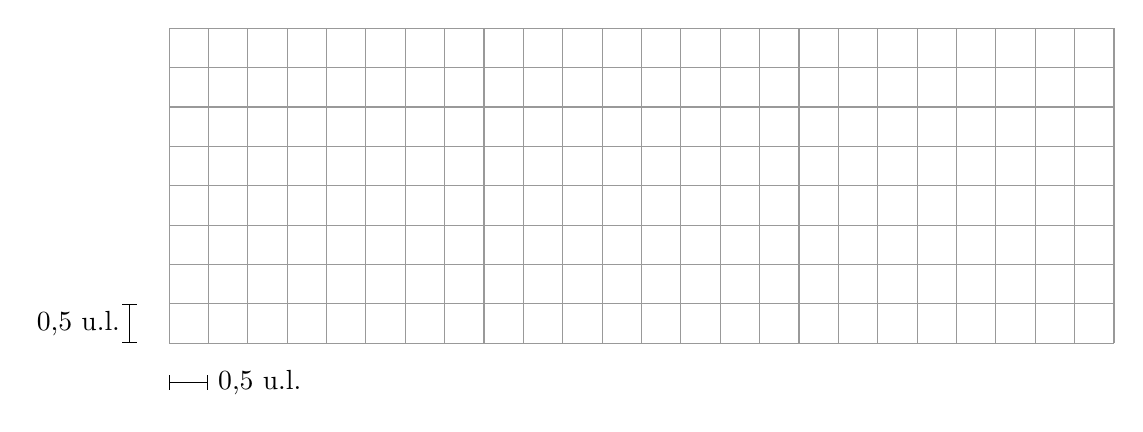
\begin{tikzpicture}
            \draw[gray!80, step=0.5] (0,0) grid (12, 4);
            \draw[|-|] (0,-.5) -- (.5,-.5)node[right]{0,5 u.l.};
            \draw[|-|] (-.5,0) -- (-.5,.5)node[midway, left]{0,5 u.l.};
        \end{tikzpicture}
    \end{center}

    \begin{enumerate}
        \item Assemble-les dans le quadrillage afin de former un seul grand
              rectangle.
        \item Quelle est l'aire de ce nouveau rectangle~? Écris ton calcul.
    \end{enumerate}
\end{exercise}

\dotsforanswer{2}[Mettre en évidence, c'est]

Exemples~:
\begin{itemize}
    \item \(5 \cdot 8 + 5 \cdot 2 =\)
    \item \(12 \cdot 3 + 6 \cdot 5 =\)
\end{itemize}

\begin{exercise}
    Effectue en utilisant la mise en évidence.
    \begin{enumerate}[cols=2, itemsep=2cm]
        \item \(8 \cdot 6 + 7 \cdot 6 =\)
        \item \(7 \cdot 21 + 3 \cdot 21 =\)
        \item \(110 \cdot 8 + 14 \cdot 8 =\)
        \item \(0,3 \cdot 7 + 7 \cdot 0,7 =\)
    \end{enumerate}
    \vspace*{2cm}
\end{exercise}

\section{Codage et décodage}

\textbf{Coder} une expression, c'est traduire en langage mathématique
une expression en français.

Exemple : La somme de 3 et de 9 vaut 12 se code par
\(\mathbf{3 + 9 = 12}\)

\textbf{Décoder} une expression, c'est traduire une expression
mathématique en français.

Exemple : \(\mathbf{72\ :8 = 9}\) se traduit par le
quotient de 72 par 8 vaut 9.

\begin{tblr}{
        hlines,
        vlines,
        row{1}={c,gray!60},
        column{1}={c,gray!60},
        cell{1}{3}={c=2}{c},
        cell{4}{1}={r=3}{}
    }
    Opérations     & Traduction en français             & Exemple                                  \\
    Addition       & La somme de \dots et \dots         & $5 + 3$     & La somme de 5 et de 3      \\
    Soustraction   & La différence entre \dots et \dots & $5 - 3$     & La différence entre 5 et 3 \\
    Multiplication & Le produit de \dots par \dots      & $5 \cdot 3$ & Le produit de 5 par 3      \\
                   & Le double de \dots                 & $2 \cdot 7$ & Le double de 7             \\
                   & Le triple de \dots                 & $3 \cdot 7$ & Le triple de 7             \\
    Division       & Le quotient de \dots par \dots     & $5 : 3$     & Le quotient de 5 par 3
\end{tblr}


\begin{exercise}
    Code les phrases suivantes.
    \begin{enumerate}
        \item Le produit de 7 par 6 vaut 42~: \dotfill.
        \item Le quotient de 54 par 9 est 6~: \dotfill.
        \item 15 est la différence entre 27 et 12~: \dotfill.
        \item La somme du triple de 8 et du double de 1~vaut 26~: \dotfill.
    \end{enumerate}
\end{exercise}
\begin{exercise}
    Décode les expressions mathématiques suivantes.
    \begin{enumerate}
        \item \dotsforanswer{2}[\(8 - 6 = 2 \rightarrow \)]
        \item \dotsforanswer{2}[\(26 : 2 = 13 \rightarrow \)]
        \item \dotsforanswer{2}[\(2 \cdot 7 + 6 = 20 \rightarrow \)]
        \item \dotsforanswer{2}[\(35 - 3 \cdot 9 = 8 \rightarrow \)]
        \item \dotsforanswer{2}[\(60 : 15 = 4 \rightarrow \)]
    \end{enumerate}
\end{exercise}

\section{Priorité des opérations}

Lorsque nous avons \emph{plusieurs opérations différentes} à effectuer
dans un même calcul, nous devons respecter un certain ordre.

Pour se rappeler de cet ordre, nous pouvons retenir \og PEMDAS \fg.
\begin{center}
    \begin{tikzpicture}
        \draw (0,0) -- (1,0) -- (1,-1) -- (2,-1) -- (2,-2) -- (3,-2) -- (3,-3) -- (4,-3) -- (4,-4);
    \end{tikzpicture}
\end{center}

Exemple~:

\(28 + 12\ :4 - (3 + 7) =\)

\begin{exercise}
    Effectue les calculs suivants en respectant la priorité des opérations. Veille à présenter correctement tes étapes~!
    \begin{enumerate}[cols=2, itemsep=3cm]
        \item \(30 - 6\ :2 =\)
        \item \(200 - 4 \cdot 16 + 5 =\)
        \item \(2 + 5 \cdot (6 + 9) =\)
        \item \((3 \cdot 12 + 5) - 10 =\)
    \end{enumerate}
    \vspace*{3cm}
\end{exercise}

\section{Exercices mélangés}
\begin{exercise}
    Vrai ou faux~? Justifie dans les deux cas.
    \begin{enumerate}
        \item L'addition est une opération associative.
        \item $-3$ fait partie de l'ensemble des naturels.
        \item 1 est un élément absorbant pour la multiplication.
        \item 0 est un élément neutre pour l'addition.
        \item Dans le calcul \(9\ :3 = 3\), \(9\) est appelé le diviseur.
    \end{enumerate}
\end{exercise}

\begin{exercise}
    Code ou décode les expressions suivantes. Ne calcule pas le résultat.
    \begin{enumerate}
        \item Le quotient de 225 par 15~
        \item Le produit de 4 par la différence entre 5 et 1
        \item La somme du triple de 2 et du double de 5
        \item \(10 - 6 = 4\)~
        \item \(2 \cdot 10 + 3 = 23\)~
        \item \((10 : 2) \cdot 3 = 15\)~
    \end{enumerate}
\end{exercise}

\begin{exercise}
    Écris le calcul qui décompose le nombre \(50\) en  \dots
    \begin{enumerate}
        \item \dots une somme de deux termes égaux
        \item \dots une différence de deux termes
        \item \dots un produit dont le premier facteur est 5
        \item \dots un quotient dont le dividende est 200~
    \end{enumerate}
\end{exercise}

\begin{exercise}
    Valentine a écrit comme calcul \og \(3 \cdot 0 \cdot 4 = 12\)\fg.
    Cyprien, à côté d'elle, lui dit qu'elle a oublié une propriété
    fondamentale de la multiplication. Qui a raison~? Explique.
\end{exercise}

\begin{exercise}
    Calcule en t'aidant de la distributivité.
    \begin{enumerate}[cols=2]
        \item \(75 \cdot 7\)
        \item \(23 \cdot 21 \)
    \end{enumerate}
\end{exercise}

\begin{exercise}
    Écris \dots

    \begin{enumerate}
        \item \dots le plus grand naturel que l'on peut écrire à l'aide de quatre chiffres différents.
        \item \dots en utilisant les chiffres 1, 8 et 7 une fois chacun, le plus petit nombre pair.
        \item \dots le plus grand naturel que l'on peut écrire à l'aide de chiffres différents.
        \item \dots \(108,090\) en supprimant un \og \(0\)\fg pour que la valeur du nombre ne change pas.
        \item \dots \(108,090\) en supprimant un \og \(0\)\fg pour que la valeur du nombre devienne la plus grande possible.
        \item \dots \(108,090\) en supprimant un \og \(0\)\fg pour que la valeur du nombre devienne la plus petite possible.
    \end{enumerate}
\end{exercise}

\begin{exercise}
    À chaque étape du calcul, identifie la propriété ou la règle utilisée.
    \begin{align*}
        54 + 125 + 246 + 75
         & = 54 + 246 + 125 + 75     \\
         & = (54 + 246) + (125 + 75) \\
         & = 300 + 200               \\
         & = 500                     \\
    \end{align*}
\end{exercise}

\begin{exercise}
    Donne le nom de la propriété utilisée dans chacune des égalités. Sois précis~!
    \begin{enumerate}[cols=2]
        \item \(3\  + \ (4\  + \ 7)\  = \ (3\  + \ 4)\  + \ 7\)
        \item \(3 \cdot 4\  + \ 3 \cdot 5\  = \ 4 \cdot 3\  + \ 5 \cdot 3\)
        \item \(4 \cdot 0 \cdot 8\  = \ 0\)
        \item \(1 \cdot 3 \cdot 322\  = \ 3 \cdot 322\)
        \item \(8 \cdot (2 \cdot 7) = \ (8 \cdot 2) \cdot 7\)
        \item \(0\  + \ 14\  = \ 14\)
        \item \(7 \cdot (8\  + \ 12) = \ (8\  + \ 12) \cdot 7\)
        \item[]
    \end{enumerate}
\end{exercise}

\begin{exercise}
    Dalya et sa sœur font des courses avec l'argent qu'elles ont gagné en
    faisant des petits jobs. Elles ont 40€ en tout. Elles veulent acheter
    un pantalon chacune, à 15 € chaque pantalon, Dalya veut acheter 3
    paires de chaussettes à 6 € la paire, et sa s\oe{}ur craque sur un collier
    à 8 €. Combien leur coutent les courses~? Écris ton calcul en une seule
    égalité.

    Ont-elles assez avec les 40€ qu'elles ont pour payer les courses~?
\end{exercise}

\begin{exercise}
    Un artisan doit réaliser cent plaques de rues numérotées de 1 à 100.
    Combien de fois devra-t-il écrire le chiffre 9 ? Explique ta réponse
    en écrivant tout ton raisonnement.
\end{exercise}

\begin{exercise}
    Marc va au marché et fait des petites courses. Il achète 3 bananes à
    0,40€ pièce, 500gr de fraises au prix de 1€ pour 100gr. Ensuite, il
    rajoute une bouteille de coca à 0,90€. Le marchand lui fait cadeau de
    0,50€. Note, en un seul calcul, ce que Marc va devoir payer, puis
    effectue.
\end{exercise}

\begin{exercise}
    Effectue en respectant la priorité des opérations.
    \begin{enumerate}[cols=4]
        \item \(13 + 9 - 5 \cdot 2\)
        \item \((6 + 2 \cdot 3) :2\)
        \item \(27 : 9 + 7 - (3 + 1)\)
        \item \(18 : 2 \cdot 3 - 7 + 8\)
    \end{enumerate}
\end{exercise}

\end{document}
